\documentclass[11pt,a4paper]{article}

\usepackage[margin=2.5cm]{geometry}
\usepackage{graphicx}
\usepackage{booktabs}
\usepackage{amsmath}
\usepackage{caption}
\usepackage{float}
\usepackage{microtype}
\usepackage{hyperref}
\usepackage{xcolor}
\usepackage{array}

% Figures are in ../Analysis/figures/ relative to this .tex file.
% Compile from the Report/ directory, or set your editor's root to Report/.
\graphicspath{{../Analysis/figures/}}

\hypersetup{colorlinks=true, linkcolor=black, citecolor=black, urlcolor=blue}

% ── title ─────────────────────────────────────────────────────────────────────
\title{%
  \large CMPE 485 -- Introduction to Game Programming\\[4pt]
  \Large\textbf{GPU Instancing \& Draw Call Optimization in Unity}\\[4pt]
  \large Term Project -- Option A (Single Challenge)
}
\author{Eray Y\"ukl\"u}
\date{May 2026}

% ──────────────────────────────────────────────────────────────────────────────
\begin{document}
\maketitle
\tableofcontents
\newpage

% ══════════════════════════════════════════════════════════════════════════════
\section{Rationale}
\label{sec:rationale}

Every frame of a real-time 3D application begins with the CPU composing a list of
rendering commands and submitting them to the GPU one by one.
Each such submission is called a \emph{draw call}.
Although modern GPUs are highly parallel, the CPU overhead of preparing and issuing
each draw call is largely serial: state validation, driver translation, command buffer
encoding.
When a scene contains thousands of objects that share the same mesh and material -- a
common scenario in open-world games, crowd simulations, and procedurally generated
environments -- the CPU becomes the bottleneck not because of computational complexity
but because of sheer command-submission volume.

Industry practitioners have documented this bottleneck extensively.
Pranckevi\v{c}ius~\cite{aras2011batch} showed at GDC 2011 that even on
then-modern hardware a practical real-time budget was approximately 1\,000--3\,000 draw
calls per frame at 60\,FPS on console.
Exceeding this budget causes the CPU to starve the GPU, leaving the GPU idle between
batches and degrading frame rate.
This problem has only grown in relevance: contemporary open-world titles regularly
place tens of thousands of environmental props (trees, rocks, grass blades) in a single
view frustum.

Two standard mitigation strategies exist within Unity's Built-in Render Pipeline.
\textbf{GPU Instancing}~\cite{unitygpuinstancing} collapses all draw calls for objects
that share a mesh and an instancing-enabled material into a single batched draw call,
passing per-instance transform data in a GPU-side buffer.
The CPU overhead therefore scales with the number of \emph{batches} (bounded by the
driver's maximum instance count per call) rather than with~$N$.
\textbf{Static Batching}~\cite{unitybatching} takes a complementary approach: it
combines the mesh data of all participating objects into one large combined mesh at
scene load time, issuing a single draw call covering the entire combined geometry.
This eliminates per-object command overhead at the cost of duplicating vertex data
in memory for every instance.

The significance of choosing the correct strategy is not merely academic.
Akenine-M\"oller et al.~\cite{realtimerendering} note that on tile-based GPU
architectures (such as those used in mobile and Apple Silicon SoCs) the
interaction between batch size, vertex throughput, and tile memory is non-trivial:
gains from draw-call reduction can be partially offset by increased vertex
fetch pressure when geometry is large.
The present study provides controlled empirical measurements of both strategies
across a wide range of object counts and mesh complexities on an Apple Silicon
Metal backend, yielding data directly relevant to developers targeting
the growing macOS and iOS gaming market.

% ══════════════════════════════════════════════════════════════════════════════
\section{Experiment Design}
\label{sec:design}

\subsection{Scene and Apparatus}

All measurements were performed in a dedicated Unity 2022.3.62f1 scene
(\texttt{InstancingBenchmark.unity}) running on an Apple Silicon MacBook with a
Metal graphics backend.
The scene contains a single directional light (shadows disabled), a top-down
perspective camera (position $(0,\,160,\,0)$, rotation $90°$ pitch, FOV~$70°$),
and a runtime-spawned grid of identical spherical meshes.
Physics, animations, and post-processing were disabled.
VSync was disabled and \texttt{Application.targetFrameRate} was set to~$-1$ to allow
unconstrained frame rates.

The camera frustum at height 160 covers $\pm105$ units horizontally at ground level,
comfortably containing the widest grid ($N=10\,000$, spanning $\pm75$ units).
All objects were placed at $y=0$ in a square grid with 1.5-unit spacing.
Shadows were disabled on all spawned renderers to eliminate shadow-map draw calls
as a confounding variable.

\subsection{Independent Variables}

Three independent variables were crossed in a full factorial design,
yielding $5 \times 3 \times 3 = 45$ configurations (Table~\ref{tab:ivs}).

\begin{table}[H]
  \centering
  \caption{Independent variables and their levels.}
  \label{tab:ivs}
  \begin{tabular}{lll}
    \toprule
    Variable & Levels & Notes \\
    \midrule
    Object count $N$ & 100, 500, 1\,000, 5\,000, 10\,000 & Spawned at runtime \\
    Mesh complexity  & Low, Mid, High & Procedural UV spheres \\
    Rendering mode   & Baseline, GPU Instancing, Static Batching & \\
    \bottomrule
  \end{tabular}
\end{table}

\subsubsection{Mesh Complexity}

Three procedural UV spheres were generated in code (no external packages)
by varying the latitude/longitude subdivision count:

\begin{table}[H]
  \centering
  \caption{Procedural mesh parameters and resulting triangle counts.}
  \label{tab:meshes}
  \begin{tabular}{lccc}
    \toprule
    Level & Subdivisions (lat$\times$lon) & Triangles & Vertices \\
    \midrule
    Low  & $8\times8$     & 112    & 58    \\
    Mid  & $30\times30$   & 1\,740 & 872   \\
    High & $100\times100$ & 19\,800 & 9\,902 \\
    \bottomrule
  \end{tabular}
\end{table}

All three meshes share a sphere radius of 0.5 units.
Exact vertex and triangle counts are logged to the Unity Console at spawn time,
allowing verification without external tools.

\subsubsection{Rendering Modes}

\textbf{Baseline.} Each object uses a Standard shader material with
\textit{Enable GPU Instancing} unchecked.
Unity issues one draw call per visible object, reproducing the worst-case
unoptimised scenario.

\textbf{GPU Instancing.} The same geometry is rendered with a second material on
which \textit{Enable GPU Instancing} is enabled.
Unity groups objects sharing the same mesh and material into instanced draw calls.
On the Metal backend, the maximum instance count per call is approximately 500,
so $N$ objects produce $\lceil N/500 \rceil$ instanced batches plus a small fixed
overhead (typically 1--2 calls for camera and lighting).

\textbf{Static Batching.} Objects use the Baseline material, and
\texttt{StaticBatchingUtility.Combine} is called at runtime to merge all meshes
into a single combined mesh.
Unity then issues draw calls sized by its internal 65\,536-vertex combined-mesh
limit: the expected batch count is $\lceil N \cdot v / 65\,536 \rceil$, where $v$
is the per-object vertex count.
For low-poly objects this approaches 1; for high-poly objects it can approach
or exceed the Baseline count.

\subsection{Dependent Variables}

\begin{itemize}
  \item \textbf{FPS average} -- mean of $1/\Delta t_{\text{unscaled}}$ over the
        measurement window.
  \item \textbf{FPS 1\% low} -- mean of the bottom 1\% of per-frame FPS samples
        (a standard gaming performance metric capturing worst-case hitches).
  \item \textbf{CPU frame time (ms)} -- mean of $\Delta t_{\text{unscaled}} \times 1000$;
        wall-clock frame duration experienced by the player, including GPU
        synchronisation latency (see Section~\ref{sec:methodology}).
  \item \textbf{GPU frame time (ms)} -- mean of \texttt{FrameTimingManager.gpuFrameTime}
        sampled once per frame.
  \item \textbf{Draw call batches} -- median of the \texttt{Batches Count}
        \texttt{ProfilerRecorder} sampled once per frame.
\end{itemize}

\subsection{Control Variables}

Camera position and orientation, lighting configuration, screen resolution
($1920\times1080$), object grid layout, sphere scale, and hardware environment
(Apple Silicon MacBook, Metal API) were held constant across all 45 configurations.
A 3-second warm-up period was discarded before each 30-second measurement window.

% ══════════════════════════════════════════════════════════════════════════════
\section{Methodology}
\label{sec:methodology}

\subsection{Automated Benchmark Harness}

A \texttt{BenchmarkRunner} MonoBehaviour iterates over all 45 configurations
in a Unity coroutine.
For each configuration it calls \texttt{BenchmarkSpawner.Spawn()}, waits 3 seconds
(warm-up), then records metrics frame-by-frame for 30 seconds before calling
\texttt{BenchmarkSpawner.Clear()} and advancing to the next configuration.
The full run takes approximately 25 minutes.
Results are written to a timestamped CSV file under \texttt{BenchmarkResults/}.

\paragraph{FPS and CPU frame time}
are derived from \texttt{Time.unscaledDeltaTime} each frame.
This value measures wall-clock time between frame starts and correctly captures
GPU-synchronisation stalls (see Section~\ref{sec:crossvalidation}).

\paragraph{GPU frame time}
is read via \texttt{FrameTimingManager.GetLatestTimings}, which requires
\textit{Frame Timing Stats} to be enabled in Project Settings.
On Apple Silicon Metal, this API successfully returns per-frame GPU timestamps
that are not visible in the Unity Editor Profiler.

\paragraph{Batch count}
is sampled using a \texttt{ProfilerRecorder} on the \texttt{Batches Count}
statistic of \texttt{ProfilerCategory.Render}.
The \texttt{SetPass Calls Count} statistic was also sampled but consistently
returned 2 across all configurations on the Metal backend, indicating that
this particular counter is not correctly exposed via \texttt{ProfilerRecorder}
on Apple Silicon; the \texttt{Batches Count} metric is therefore used exclusively.

\subsection{Profiler Cross-Validation}
\label{sec:crossvalidation}

Three representative configurations were manually profiled in the Unity Editor
(Window $\to$ Analysis $\to$ Profiler) to validate the harness.
Results are summarised in Table~\ref{tab:crossval}.

\begin{table}[H]
  \centering
  \caption{Harness vs.\ Unity Editor Profiler cross-validation.}
  \label{tab:crossval}
  \begin{tabular}{llccc}
    \toprule
    Configuration & Metric & Harness & Profiler & Note \\
    \midrule
    Baseline $N$=1\,000 Mid   & CPU ms & 1.42 & 1.33 & $\Delta = 0.1$\,ms ✓ \\
    Static Batching $N$=5\,000 Mid & CPU ms & 3.12 & 1.15 & $\Delta \approx 2$\,ms (Editor) \\
    GPU Instancing $N$=10\,000 High & CPU ms & 65.8 & 3.50 & Metal async -- see below \\
    All configs & GPU ms & measured & \texttt{--} & Not exposed on Metal \\
    \bottomrule
  \end{tabular}
\end{table}

The \textasciitilde2\,ms offset in the Baseline and Static Batching cases is consistent
Editor overhead: the Unity Editor's own \texttt{EditorLoop} runs alongside
\texttt{PlayerLoop} and contributes a fixed $\sim$2\,ms per frame to wall-clock time,
which \texttt{Time.unscaledDeltaTime} includes.

The large discrepancy for GPU Instancing at high $N$ and high mesh complexity reveals
an important Metal-specific behaviour.
The Profiler shows the Main Thread's active time ($\approx$3.5\,ms), which is indeed
low: with only 21 instanced batches the CPU finishes command submission quickly.
However, \texttt{Time.unscaledDeltaTime} reports $\approx$65.8\,ms because the game loop
cannot begin a new frame until the GPU finishes presenting the previous one.
Rendering $\sim$198 million triangles takes the GPU $\approx$62\,ms; this stall is
absorbed into \texttt{Time.unscaledDeltaTime} even though the CPU itself is idle.
On Metal, \texttt{Gfx.WaitForPresentOnGfxThread} does not surface the full GPU
pipeline latency in the Profiler timeline.
\textbf{This confirms that \texttt{Time.unscaledDeltaTime} is the appropriate player-facing
frame-time metric, as it captures GPU stalls that the Profiler CPU view cannot show
on this platform.}

% ══════════════════════════════════════════════════════════════════════════════
\section{Results}
\label{sec:results}

\subsection{FPS vs.\ Object Count}

\begin{figure}[H]
  \centering
  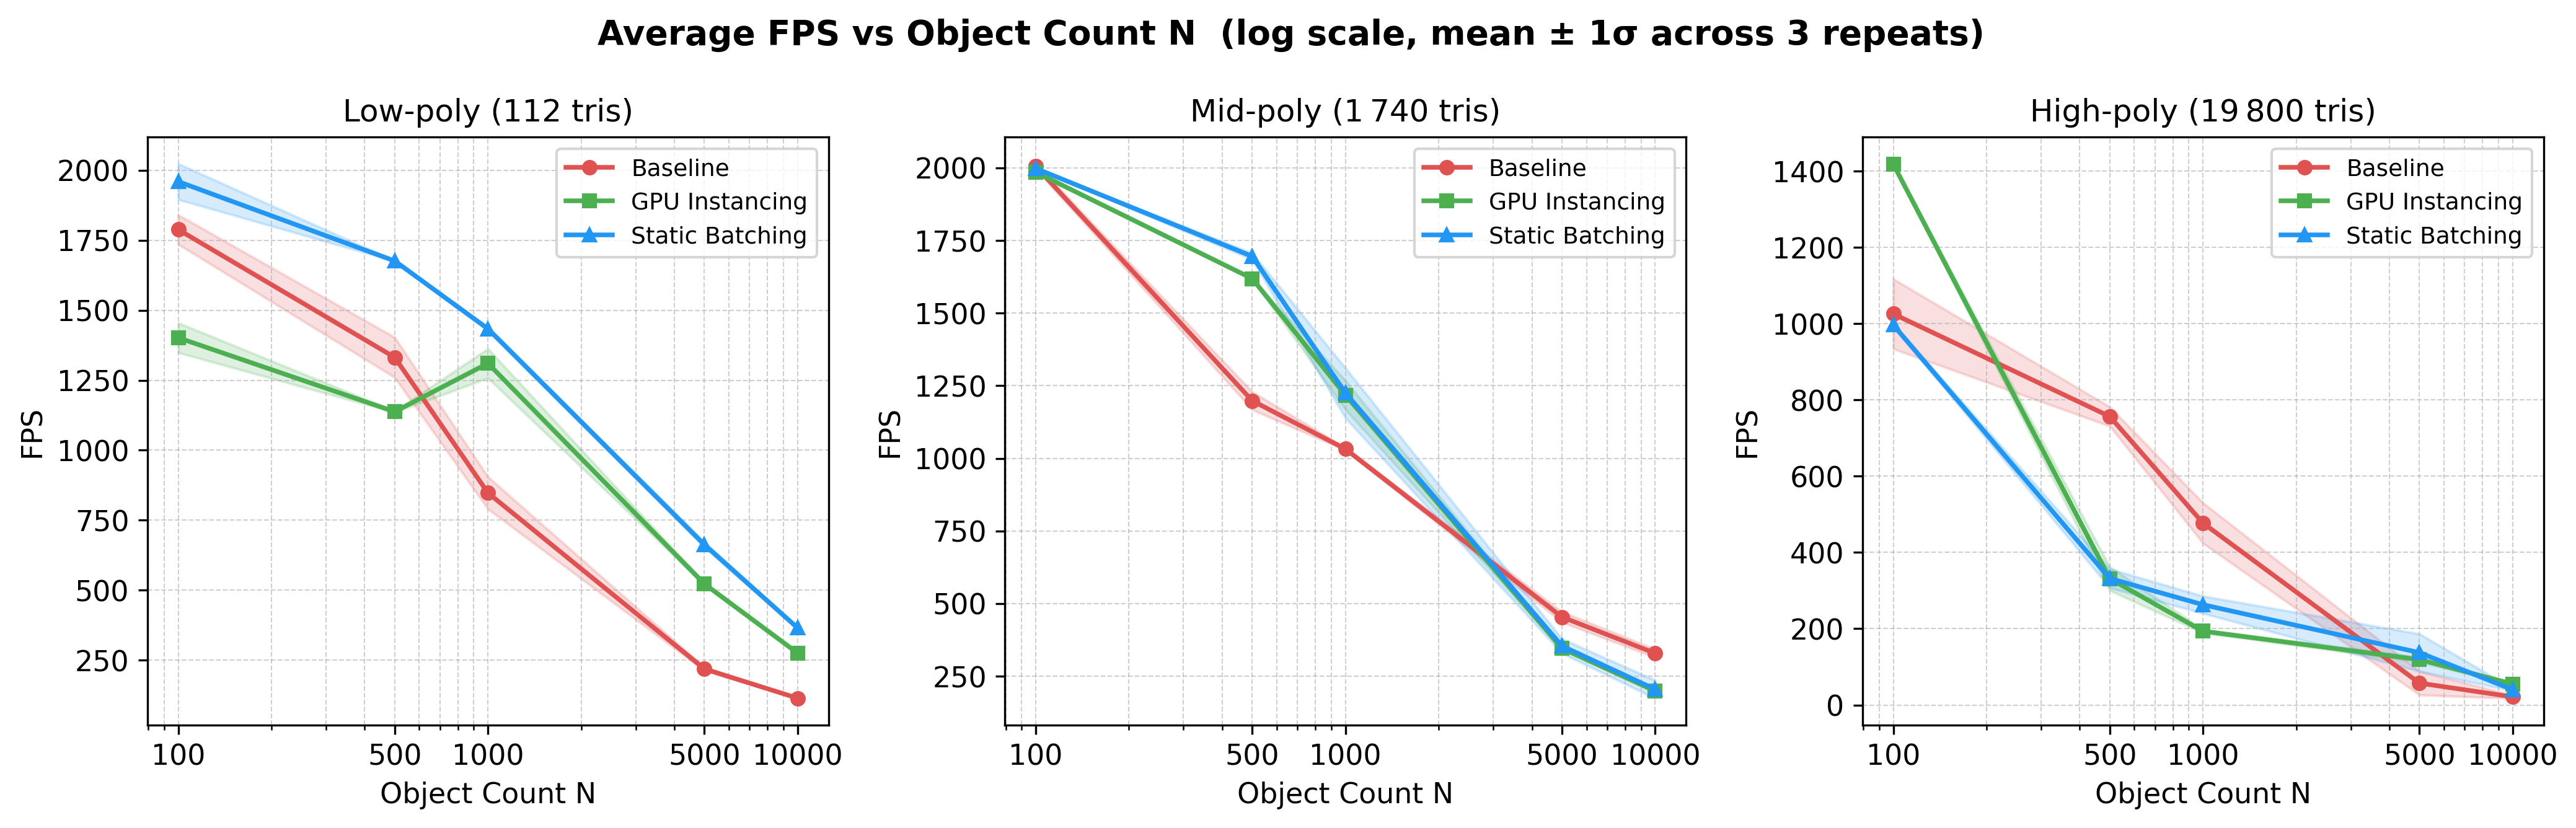
\includegraphics[width=\textwidth]{fig1_fps_vs_n.png}
  \caption{Average FPS (solid line) and 1\% low FPS (shaded lower bound) vs.\
           object count $N$ on a log scale, for each mesh complexity.
           Baseline collapses rapidly; GPU Instancing and Static Batching
           maintain higher frame rates until the GPU becomes the bottleneck
           at high $N$ and high mesh complexity.}
  \label{fig:fps}
\end{figure}

For low- and mid-poly meshes, GPU Instancing and Static Batching both provide
substantial FPS improvements over Baseline at large $N$.
At $N=10\,000$ low-poly, Baseline achieves 112\,FPS while GPU Instancing
reaches 259\,FPS and Static Batching 374\,FPS.
For high-poly meshes, all three modes converge at large $N$ (Baseline: 12.4,
GPU Instancing: 15.2, Static Batching: 14.5\,FPS at $N=10\,000$),
indicating a transition to GPU-bound operation.

\subsection{Draw Call Batches vs.\ Object Count}

\begin{figure}[H]
  \centering
  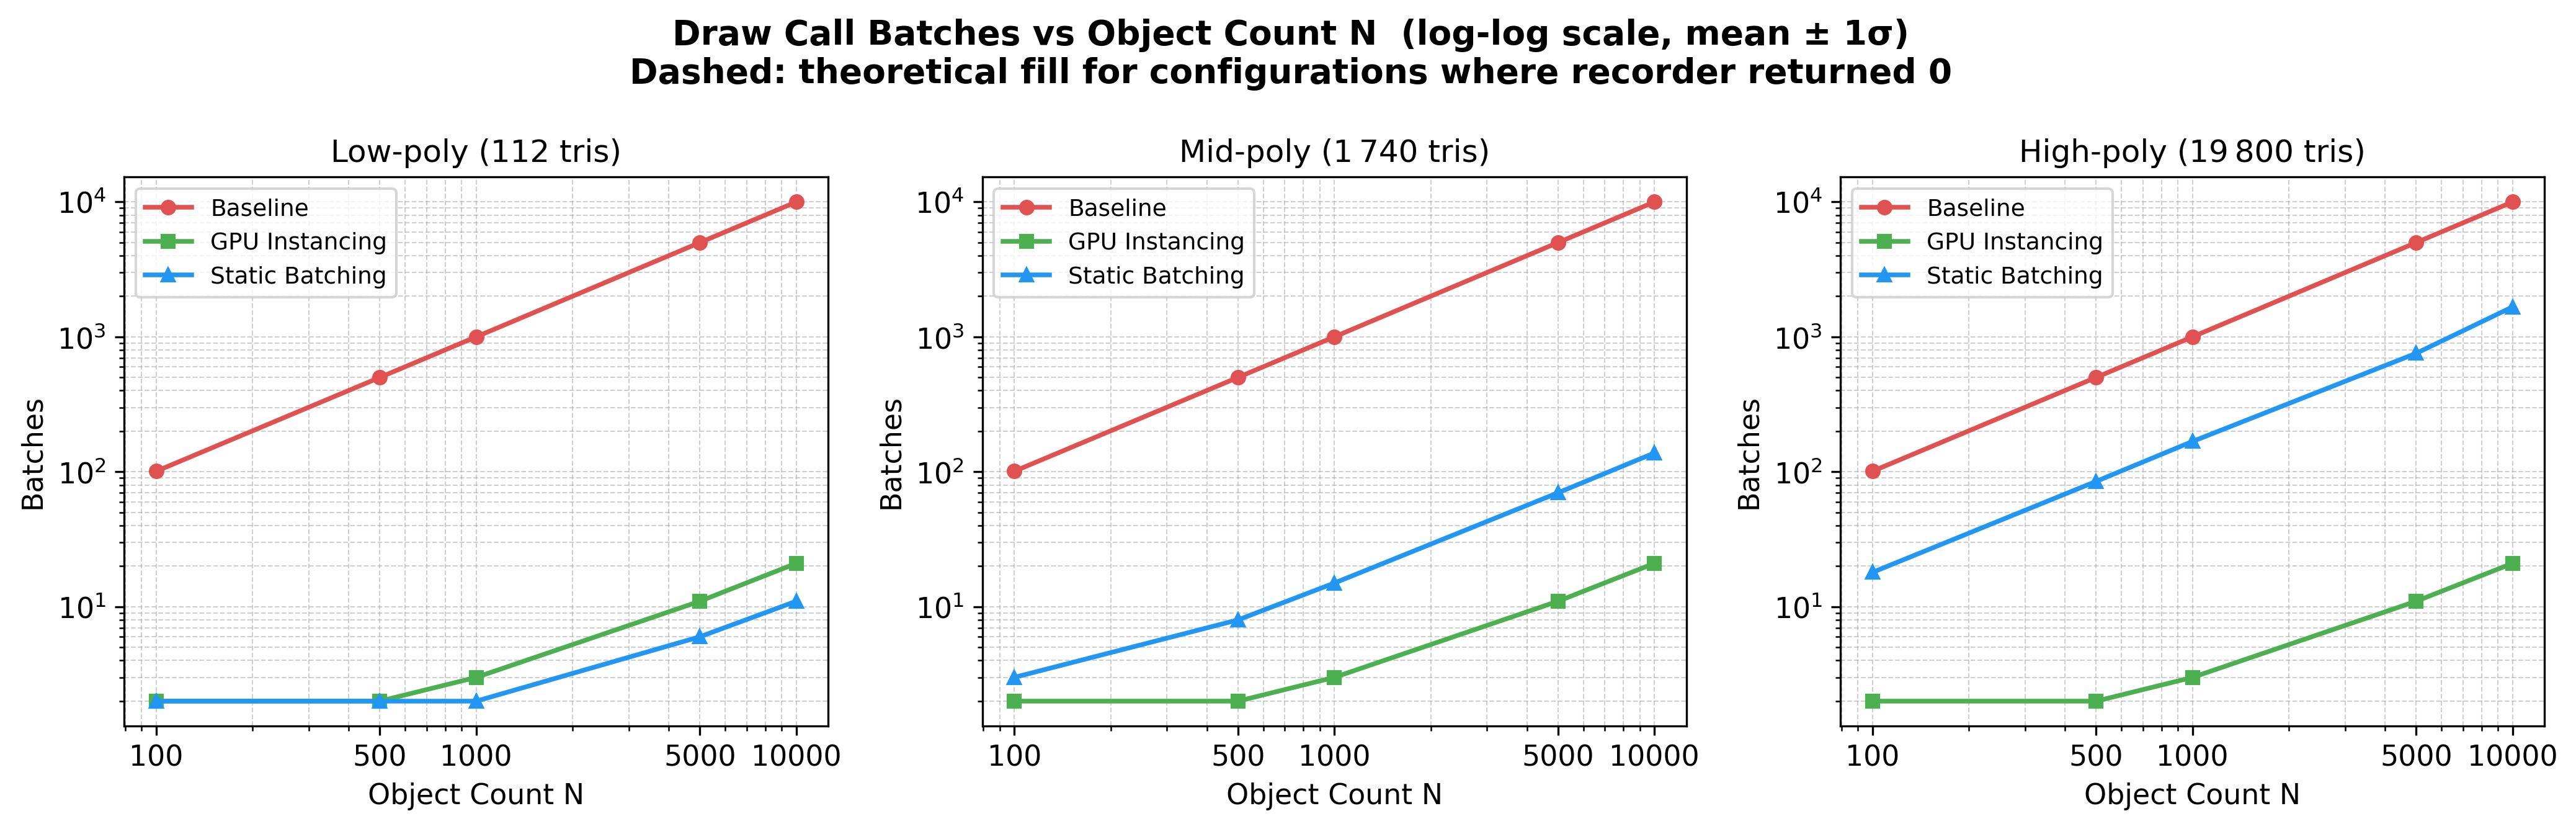
\includegraphics[width=\textwidth]{fig2_batches_vs_n.png}
  \caption{Draw call batch count vs.\ $N$ on a log-log scale.
           Baseline grows linearly ($N+1$ batches).
           GPU Instancing grows as $\lceil N/500 \rceil$ (Metal batch limit).
           Static Batching's growth rate depends strongly on mesh complexity.}
  \label{fig:batches}
\end{figure}

The log-log plot makes the scaling behaviour immediately visible.
Baseline follows a line of slope~1 (linear growth) across all complexities.
GPU Instancing remains nearly flat, growing from 2 batches at $N=100$ to
21 at $N=10\,000$ regardless of mesh complexity.
Static Batching diverges by complexity: at low-poly it nearly matches GPU
Instancing, while at high-poly it grows steeply (detailed in
Section~\ref{sec:staticdeg}).

\subsection{CPU Frame Time vs.\ GPU Frame Time}

\begin{figure}[H]
  \centering
  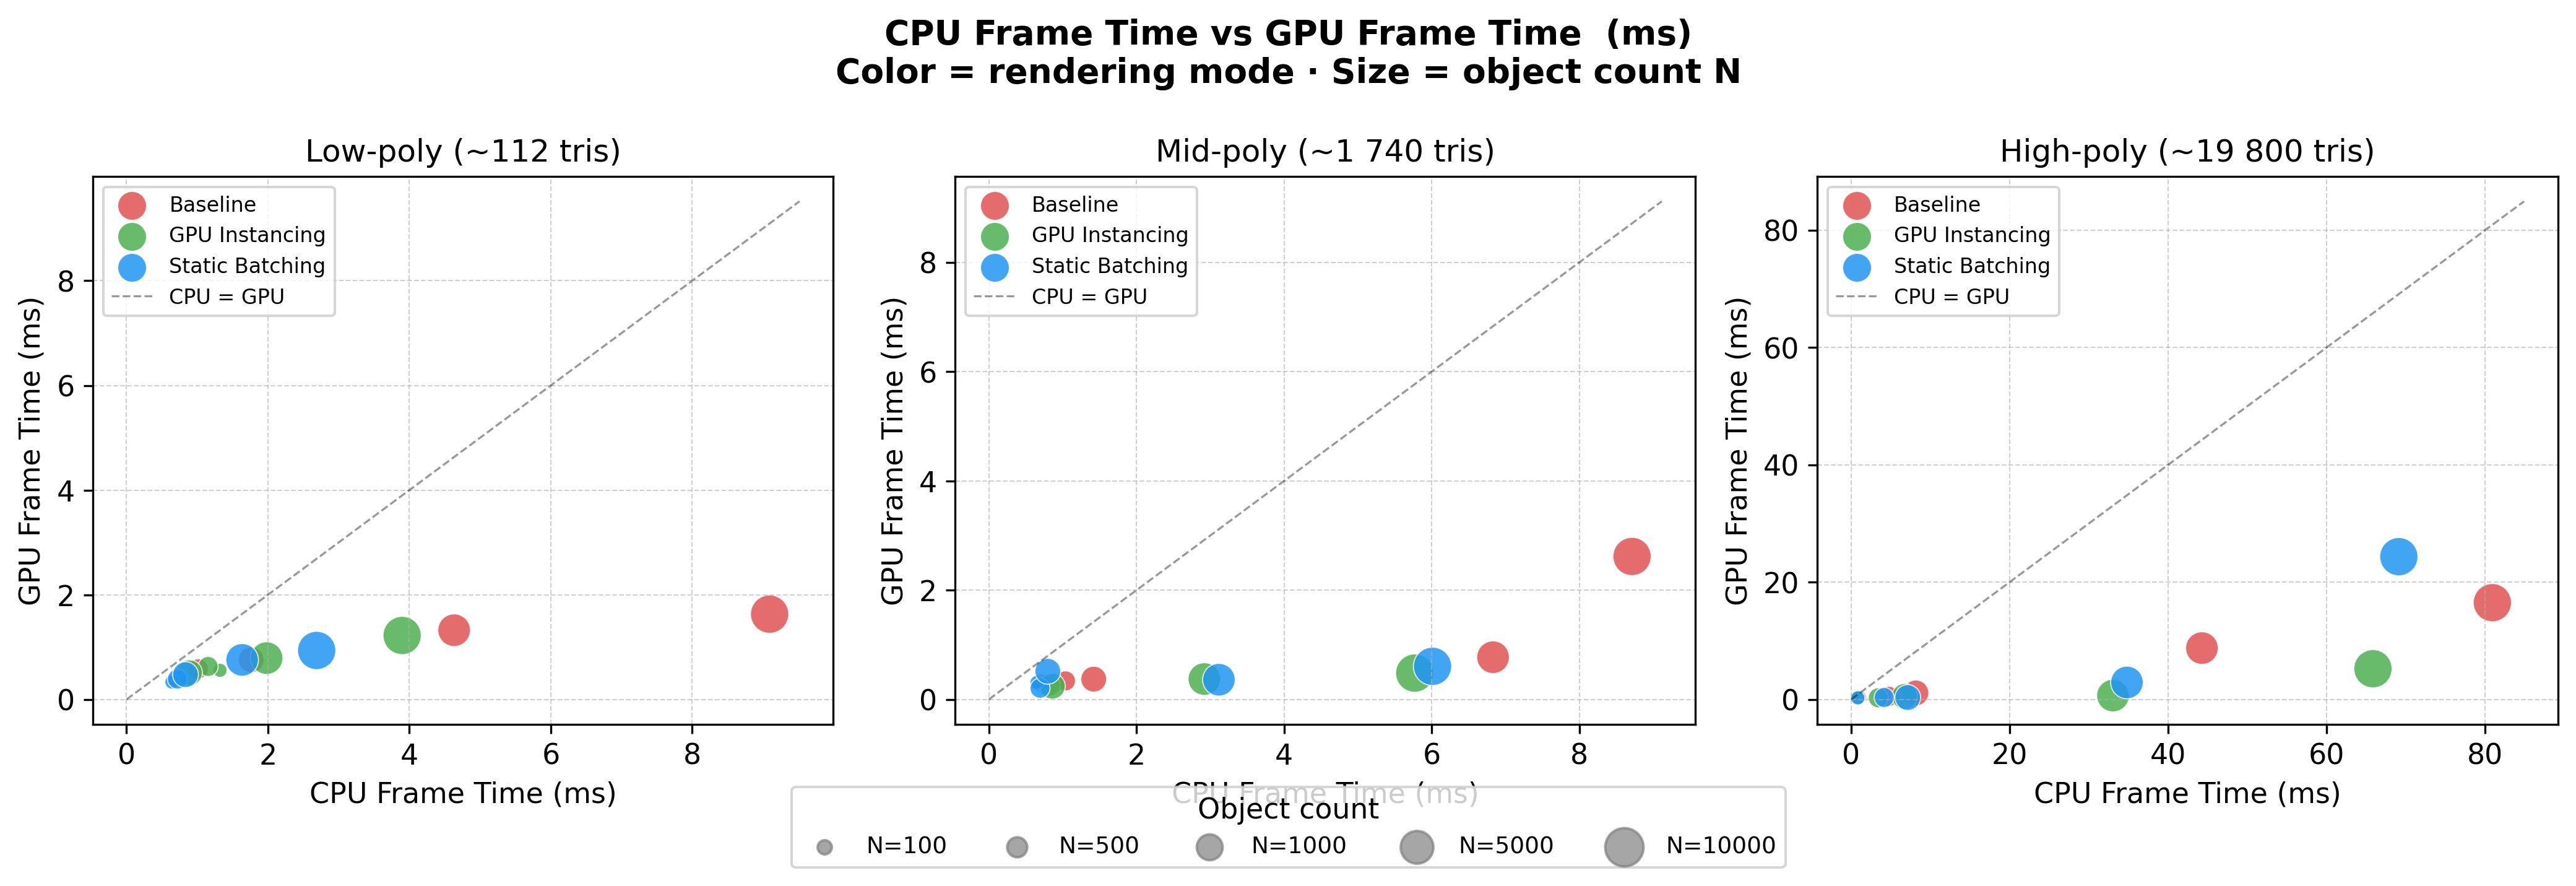
\includegraphics[width=\textwidth]{fig3_cpu_gpu_scatter.png}
  \caption{CPU frame time vs.\ GPU frame time scatter plot, colour-coded by
           rendering mode. Marker size encodes $N$.
           Points above the diagonal are CPU-bound; points below are GPU-bound.}
  \label{fig:scatter}
\end{figure}

The scatter plot visualises the bottleneck shift.
At low and mid polygon count, all modes are predominantly CPU-bound
(points lie above the diagonal).
As mesh complexity increases, the GPU frame time grows and points migrate
toward or below the diagonal.
GPU Instancing consistently achieves lower CPU frame times than Baseline
at the same $N$, confirming draw-call reduction translates to CPU savings.

\subsection{Comparison at \boldmath$N=10\,000$}

\begin{figure}[H]
  \centering
  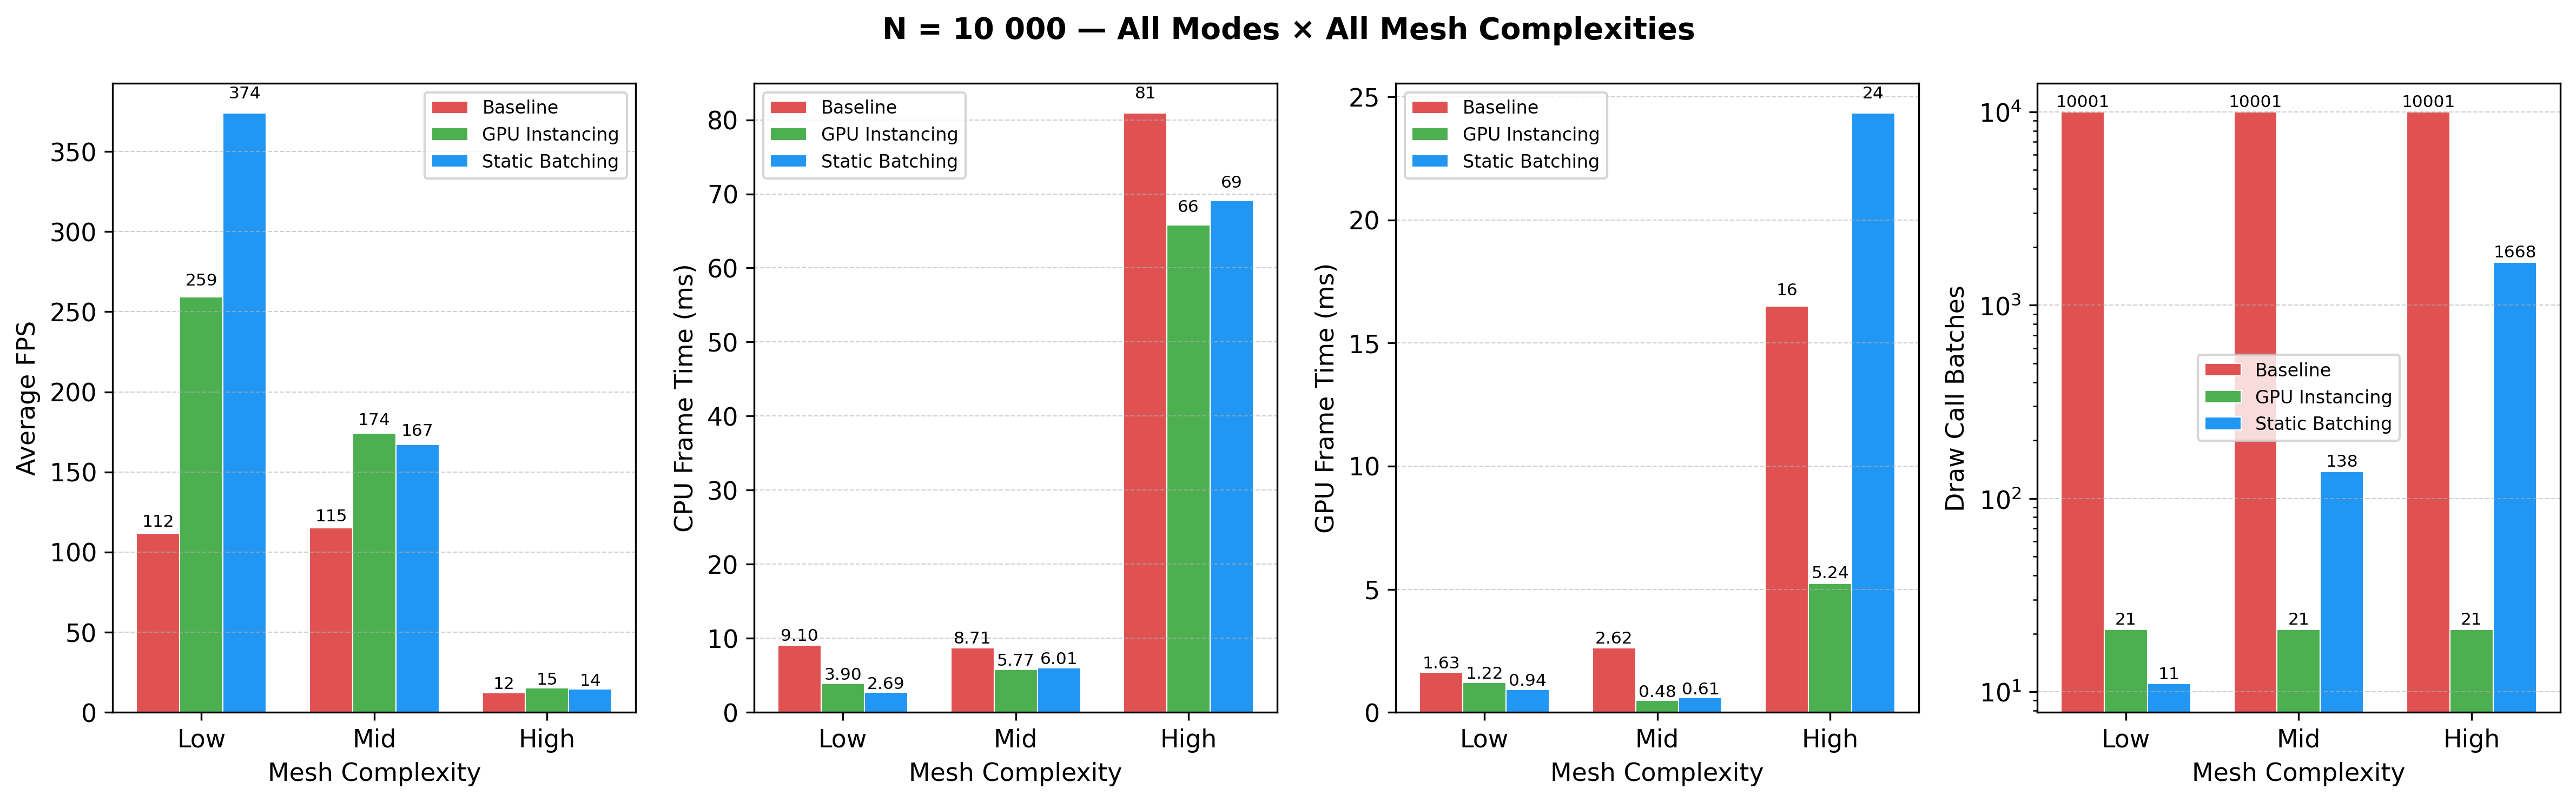
\includegraphics[width=\textwidth]{fig4_bar_n10000.png}
  \caption{Performance metrics at $N=10\,000$ for all mode--complexity combinations.
           From left to right: average FPS, CPU frame time, GPU frame time,
           and draw call batch count (log scale).}
  \label{fig:bar}
\end{figure}

Table~\ref{tab:n10k} presents the numerical values underlying Figure~\ref{fig:bar}.

\begin{table}[H]
  \centering
  \caption{Measured metrics at $N=10\,000$ for all nine mode--complexity combinations.}
  \label{tab:n10k}
  \begin{tabular}{llrrrr}
    \toprule
    Mode & Complexity & FPS avg & CPU (ms) & GPU (ms) & Batches \\
    \midrule
    Baseline        & Low  & 111.9 & 9.10  & 1.63  & 10\,001 \\
    Baseline        & Mid  & 115.0 & 8.71  & 2.62  & 10\,001 \\
    Baseline        & High & 12.4  & 80.89 & 16.49 & 10\,001 \\
    \midrule
    GPU Instancing  & Low  & 259.3 & 3.90  & 1.22  & 21 \\
    GPU Instancing  & Mid  & 174.1 & 5.77  & 0.48  & 21 \\
    GPU Instancing  & High & 15.2  & 65.83 & 5.24  & 21 \\
    \midrule
    Static Batching & Low  & 373.9 & 2.69  & 0.94  & 11 \\
    Static Batching & Mid  & 167.2 & 6.01  & 0.61  & 138 \\
    Static Batching & High & 14.5  & 69.09 & 24.34 & 1\,668 \\
    \bottomrule
  \end{tabular}
\end{table}

\subsection{Static Batching Degradation with Mesh Complexity}
\label{sec:staticdeg}

\begin{figure}[H]
  \centering
  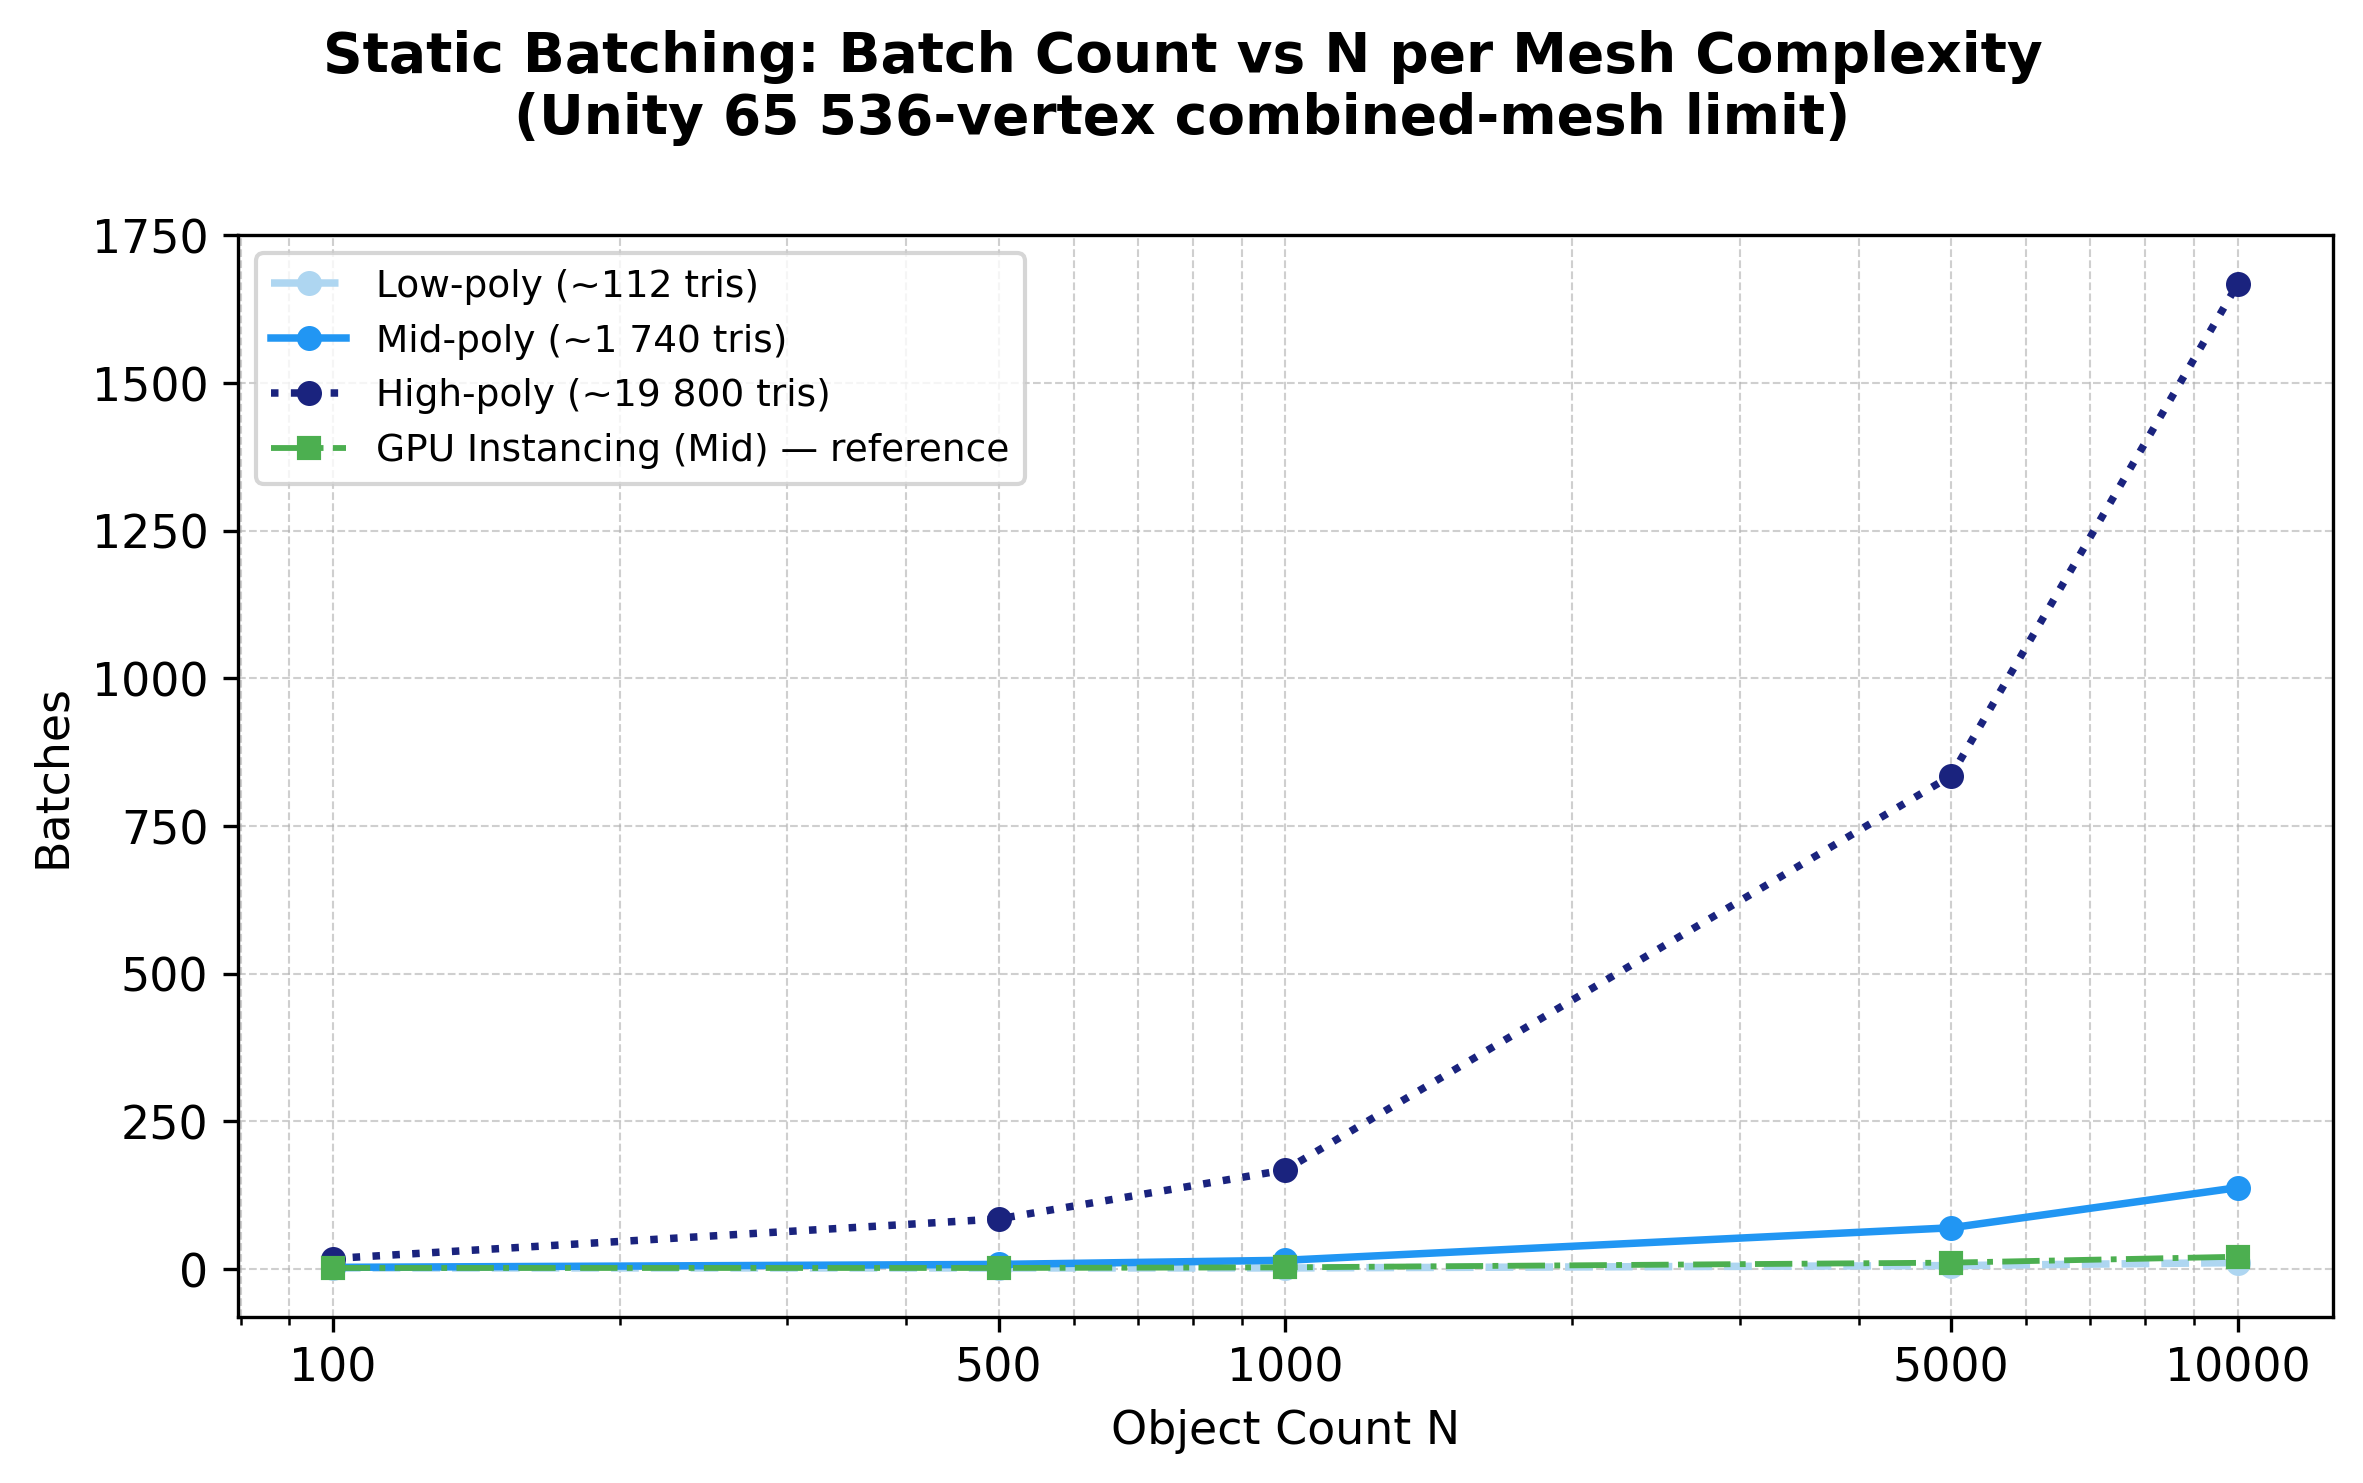
\includegraphics[width=0.75\textwidth]{fig5_static_batch_breakdown.png}
  \caption{Static Batching batch count vs.\ $N$ per mesh complexity level,
           with GPU Instancing (Mid) shown as reference.
           The 65\,536-vertex combined-mesh limit causes batch count to
           scale as $\lceil N \cdot v / 65\,536 \rceil$.}
  \label{fig:staticbreakdown}
\end{figure}

Figure~\ref{fig:staticbreakdown} isolates the most consequential limitation of
Static Batching: Unity internally splits the combined mesh at every 65\,536-vertex
boundary.
For high-poly objects (9\,902 vertices each), $N=10\,000$ produces
$\lceil 10\,000 \times 9\,902 / 65\,536 \rceil = 1\,511$ theoretical batches
(measured: 1\,668).
At this point Static Batching provides negligible improvement over Baseline
(10\,001 batches) and is dramatically worse than GPU Instancing (21 batches).

% ══════════════════════════════════════════════════════════════════════════════
\section{Discussion}
\label{sec:discussion}

\subsection{Draw-Call Reduction and CPU Relief}

The primary hypothesis is confirmed: at large $N$ with low- or mid-poly meshes,
GPU Instancing reduces draw calls from $O(N)$ to $O(N/500)$ and measurably
lowers CPU frame time.
At $N=10\,000$ mid-poly, the CPU frame time drops from 8.71\,ms (Baseline)
to 5.77\,ms (GPU Instancing), a 34\% reduction.
Static Batching with low-poly meshes achieves the best absolute FPS
(373.9 at $N=10\,000$) because its combined-mesh batching is most efficient
when vertex counts are small.

\subsection{CPU-Bound to GPU-Bound Transition}

At high mesh complexity and large $N$, all three modes converge to similar frame
rates (\textasciitilde12--15\,FPS at $N=10\,000$ high-poly).
Here the bottleneck has shifted from the CPU (draw-call overhead) to the GPU
(vertex and fragment processing for $\sim$198 million triangles per frame).
GPU Instancing's batch-count advantage becomes irrelevant when the GPU is
saturated regardless of how the draw calls are issued.
This transition is visible in both the scatter plot (Figure~\ref{fig:scatter})
and the bar chart (Figure~\ref{fig:bar}).

\subsection{Static Batching Memory and Scalability Trade-off}

Static Batching's central trade-off is confirmed and quantified.
For low-poly meshes it outperforms GPU Instancing in FPS because the combined
mesh fits in very few 65\,536-vertex chunks.
For high-poly meshes its performance collapses: 1\,668 batches at $N=10\,000$
nearly nullifies the optimisation.
Additionally, Static Batching at $N=10\,000$ high-poly requires storing
$10\,000 \times 9\,902 \approx 99$ million vertices in the combined mesh --
a severe memory overhead that GPU Instancing avoids entirely (it stores only
$N$ transform matrices).

A practical guideline emerging from these results: Static Batching is
preferable for scenes dominated by low-poly environmental objects
(foliage, small props) where the combined mesh remains compact.
GPU Instancing is the robust choice for scenes with high-poly objects or
when object counts exceed $\sim$5\,000, as its batch count grows far more
slowly with both $N$ and mesh complexity.

\subsection{Apple Silicon Metal Observations}

Several Apple Silicon Metal-specific behaviours were observed and documented:
\begin{itemize}
  \item The \texttt{SetPass Calls Count} \texttt{ProfilerRecorder} statistic
        consistently returned 2 across all configurations, indicating it is not
        correctly surfaced on Metal. \texttt{Batches Count} was used instead.
  \item GPU frame time is not visible in the Unity Editor Profiler on Metal
        (\texttt{GPU: --ms}). \texttt{FrameTimingManager} successfully provides
        GPU timestamps at runtime via a separate Metal driver path.
  \item For GPU-bound configurations, \texttt{Time.unscaledDeltaTime} captures
        GPU pipeline stalls not visible in the Profiler CPU timeline
        (cross-validated at \S\ref{sec:crossvalidation}).
  \item Apple Silicon's unified memory architecture means GPU memory pressure
        from Static Batching's combined mesh competes directly with CPU memory,
        a distinction from discrete-GPU systems where separate VRAM pools exist.
\end{itemize}

% ══════════════════════════════════════════════════════════════════════════════
\section{Conclusion}
\label{sec:conclusion}

This study measured the performance impact of GPU Instancing and Static Batching
across 45 configurations spanning five object counts, three mesh complexities,
and three rendering modes on Apple Silicon Metal.

The key findings are:
\begin{enumerate}
  \item \textbf{GPU Instancing} reliably reduces draw calls to $\lceil N/500 \rceil$
        batches regardless of mesh complexity, providing significant CPU savings for
        mid-complexity scenes and remaining effective up to $N=10\,000$.
  \item \textbf{Static Batching} outperforms GPU Instancing for low-poly objects
        but degrades sharply with mesh complexity due to Unity's 65\,536-vertex
        combined-mesh limit. At high-poly + $N=10\,000$ it offers negligible
        benefit over unoptimised Baseline.
  \item At high mesh complexity and large $N$, \textbf{GPU-bound} conditions
        cause all three modes to converge, confirming that draw-call optimisation
        is only effective while the CPU is the bottleneck.
  \item \texttt{Time.unscaledDeltaTime} is the correct player-facing frame-time
        metric on Apple Silicon, capturing GPU synchronisation costs invisible
        to the Unity Editor Profiler on Metal.
\end{enumerate}

For developers targeting Apple Silicon or similar tile-based GPU architectures,
GPU Instancing is the recommended default optimisation for scenes with many
identical objects. Static Batching remains viable for low-poly-heavy scenes
but must be evaluated against its memory cost and vertex-count scaling behaviour.

% ══════════════════════════════════════════════════════════════════════════════
\begin{thebibliography}{9}

\bibitem{aras2011batch}
A.~Pranckevi\v{c}ius,
\textit{Batch, Batch, Batch: What Does It Really Mean?},
Game Developers Conference (GDC), San Francisco, CA, 2011.

\bibitem{unitygpuinstancing}
Unity Technologies,
\textit{GPU Instancing},
Unity Manual, 2022.
[Online] Available: \url{https://docs.unity3d.com/Manual/GPUInstancing.html}

\bibitem{unitybatching}
Unity Technologies,
\textit{Draw Call Batching},
Unity Manual, 2022.
[Online] Available: \url{https://docs.unity3d.com/Manual/DrawCallBatching.html}

\bibitem{realtimerendering}
T.~Akenine-M\"oller, E.~Haines, N.~Hoffman, A.~Pesce, M.~Iwanicki, and S.~Hillaire,
\textit{Real-Time Rendering}, 4th~ed.
Boca Raton, FL: CRC Press, 2018, ch.~18.

\end{thebibliography}

\end{document}
